\section{An exact interpolant audit of portable PSM data}
\label{sec:real-admissibility}
Use \texttt{psm\_temperature\_2500}, with 340 measured operating points at
each rotor reference 30 and 70 $^\circ$C. The manifest records raw source hash,
grouping, resistance and measured electrical-speed inversion. Edited speed
variants are excluded. Terminal currents are the numerical arguments; whether
they are storage-conjugate magnetic currents is a physical assumption to test.

\subsection{Remove quadrature error, retain the interpolation limitation}
Triangulate measured currents and interpolate each flux component affinely.
Inside a triangle the flux Jacobian is constant. Split every path segment at
all intersected mesh edges and integrate each affine piece by its midpoint:
the integral is exact for that piecewise-affine field. Independently clip
triangles against each tested rectangle and sum their curl times clipped area,
with the rectangle orientation retained. This second route implements Green's
theorem without using the path calculation.

Choose the path origin as the mean of the five smallest-current points in
each slice, a support-contained reference whose coordinates are stored in the
numerical report. Compare d-then-q and q-then-d paths to every third point,
excluding locations near either translated axis. Both corners and edges must
remain inside the convex hull. The resulting paths are selected support tests,
not an exhaustive bound on every loop.

\begin{table}[htbp]\centering\small
\begin{tabular}{rrrrrr}
\toprule
Ref. / $^\circ$C & Curl all & Curl cond.$\le10$ & Paths & Path RMS & Green error\\
\midrule
30 & 6.902 & 0.042 & 86 & 1.064 & 8.1e-15 \\
70 & 9.051 & 0.039 & 85 & 0.933 & 6.2e-15 \\
\bottomrule
\end{tabular}

\caption{Exact P1 audit. Curl RMS is area-weighted in mH. Path RMS and the
maximum independent Green discrepancy are in normalized co-energy joules.}
\end{table}
Path disagreement is about one joule under the fixed dq normalization, while
the two exact integration routes agree near floating-point precision.
The interpolated field therefore fails to be an exact common gradient.
The Green agreement removes an integration implementation error as an
explanation; it does not remove interpolation bias or measurement uncertainty.

\subsection{Local derivatives need a geometric sensitivity check}
Very thin triangles amplify flux differences into large gradients.
Report all triangles and the sensitivity subset whose two-edge matrix has
condition at most 10. Area-weighted curl RMS changes substantially under this
mask, so the unmasked local derivative magnitude is not a stable physical
estimate. The mask is a sensitivity experiment, not a residual-based deletion.
Closed paths integrate larger regions and expose another scale of inconsistency.
\begin{figure}[htbp]\centering
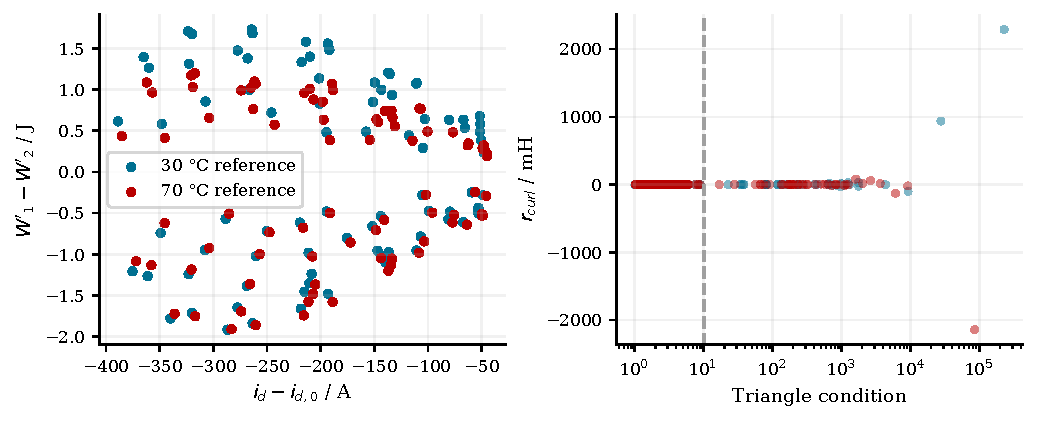
\includegraphics[width=\textwidth]{figures/real_integrability.pdf}
\caption{Left: signed path disagreement for supported rectangles. Right:
triangle curl versus geometric condition. The dashed threshold marks the
reported geometric sensitivity subset.}
\label{fig:real-integrability}\end{figure}

An affine conservative reference on an independently generated square mesh
has zero curl and path disagreement to roundoff. It checks signs and exact
integration where interpolation reproduces the known field. For curved real
fields, P1 interpolation itself can violate reciprocity; the measured result
cannot assign the full observed discrepancy to the underlying machine.
